% Figure M4 hero prototype : generated by experiments/m4_facet_vs_sae.py --hero.
% Preview-only; not yet linked from the main manuscript.
\begin{figure}[t]
 \centering
 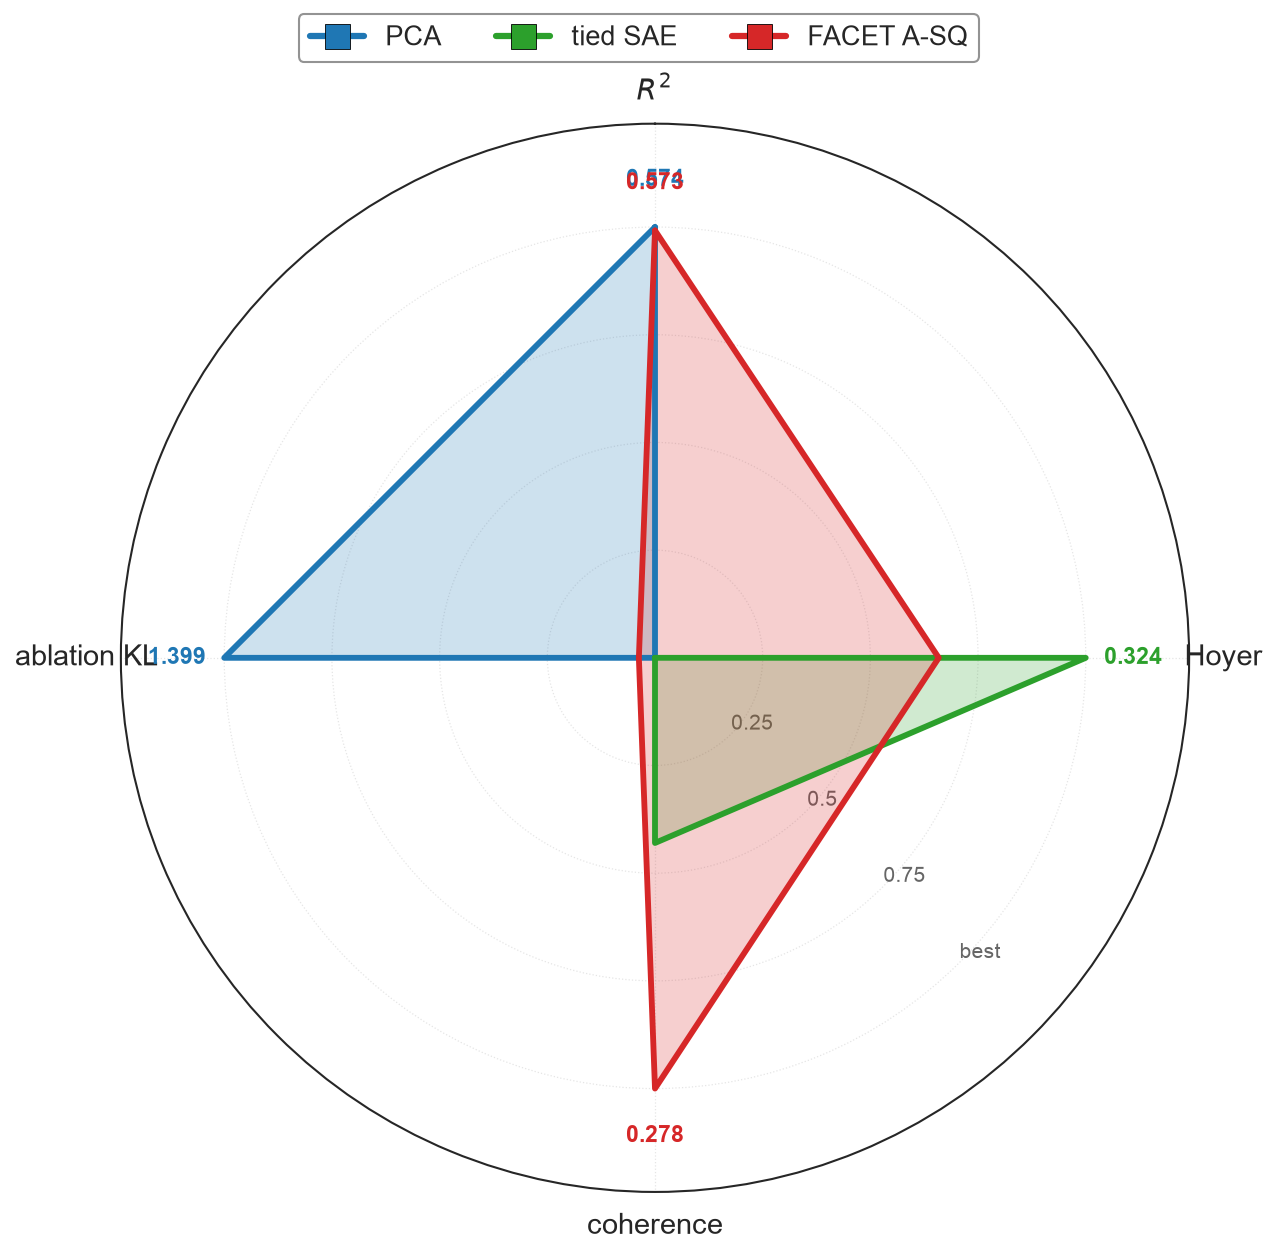
\includegraphics[width=\linewidth]{../shared/figures/generated/m4_facet_vs_sae_hero.png}
 \caption{\textbf{M4 hero: three-way representation / sparsity / causal trade-off at matched $m{=}32$.} GPT-2 small block~4 \texttt{attn\_out}. \textbf{(a)}~Radar of the four M4 metrics ($R^2$, Hoyer, top-token coherence, ablation KL) rescaled to $[0,1]$ by $(v-\min)/(\max-\min)$ across the three methods; a vertex at the outer ring means the method is best on that axis. Numeric raw values are annotated at every per-axis winner. \textbf{(b)}~Grouped bars at raw units with numeric labels, provided so the actual values do not have to be decoded from the radar. FACET A-SQ reaches a vertex on $R^2$ (tied with PCA) and on top-token coherence; PCA reaches a vertex on ablation KL; the tied SAE reaches a vertex on Hoyer sparsity and pays the $R^2$ cost that FACET's threshold operator avoids.}
 \label{fig:m4-facet-vs-sae-hero}
\end{figure}
